\selectlanguage{english}
\appendice{Probabilités de transition entre réseaux trophiques}
\label{annIII}
\addtocounter{chapter}{1}
\setcounter{equation}{0}


La TTIB proposée par \cite{Gravel2011} est issue d'une collaboration entre cinq auteurs~:
Dominique Gravel, François Massol, Elsa Canard, David Mouillot et Nicolas Mouquet.
Parmi ces auteurs, Francois Massol a récemment été invité à soumettre une
contribution au volume 56 du journal scientifique
\emph{Advances in Ecological Research} traitant du lien entre les réseaux
écologiques et l'invasion des espèces, volume dont il est coéditeur.
Ce fut une opportunité pour montrer les possibilités offertes par la TTIB et aussi
une occasion de pouvoir revenir en détail sur les mathématiques en arrière du modèle.
L'article final, est une collaboration entre François Massol
(premier auteur), Maxime Dubart, Vincent Calcagno, Claire Jacquet, Sonia Kéfi,
Dominique Gravel (dernier auteur) et moi-même.

C'est pour mon travail sur l'extension de la TIB présenté au chapitre \ref{chap1}
que j'ai été invité à contribuer à cet article. Ma participation détaille
quelques aspects techniques du modèle mathématique ainsi que les nouvelles
possibilités qu'il ajoute à la TIB.
Dans cette annexe, je présente mon travail tel qu'il était avant d'être intégré
dans l'article qui est actuellement en cours de révision.
La figure qui y est présentée est de Francois Massol qui m'a gentiment permis
de la réutiliser. La notation $P_{X}$ représente la probabilité de l'événement
$X$, c'est donc l'équivalent de la notation $\mathbb{P}(X)$ à l'annexe \ref{annII}.



\section{The model}\label{the-model}

An alternative to study analytically the model of the TTIB proposed by \cite{Gravel2011}
is to derive master equations associated to community states (rather than for individual species).
The mathematical object is then the random process
$(C_{t>0}=\cup_{i=1}^TX_i$, \emph{i.e.} a vector of 0 and 1 describing
the presence and absence of all species at any time \(t\). For \(T\)
species, there are \(2^T\) community states, Table \ref{tabAnnIII_1} provides an example
for species B, C, D and E presented in Figure \ref{ann3fig1} .


\begin{table}[]
\centering
\caption[Community states associated to simple networks]{Community states
associated to the B-C-D-E network of figure \ref{ann3fig1}. They represent
all combinations of presence and absence of species. At any time
\(t\), \(C_{t>0}\) represents the species composition of the island and
thus is in one of the sixteen possible \(S_k\) states listed. Here, all
communities are considered regardless whether or not they are TTIB-compatible
as highlighted in the right column.}
\label{tabAnnIII_1}
  \begin{tabular}{|l|l|l|l|l|l|}
    Community states & B & C & D & E & TTIB-compatible \\ \hline
    \(S_{0}\) & 0 & 0 & 0 & 0 & yes \\
    \(S_{1}\) & 0 & 0 & 0 & 1 & no \\
    \(S_{2}\) & 0 & 0 & 1 & 0 & yes \\
    \(S_{3}\) & 0 & 0 & 1 & 1 & yes \\
    \(S_{4}\) & 0 & 1 & 0 & 0 & yes \\
    \(S_{5}\) & 0 & 1 & 0 & 1 & yes \\
    \(S_{6}\) & 0 & 1 & 1 & 0 & yes \\
    \(S_{7}\) & 0 & 1 & 1 & 1 & no \\
    \(S_{8}\) & 1 & 0 & 0 & 0 & no \\
    \(S_{9}\) & 1 & 0 & 0 & 1 & no \\
    \(S_{10}\) & 1 & 0 & 1 & 0 & no \\
    \(S_{11}\) & 1 & 0 & 1 & 1 & yes \\
    \(S_{12}\) & 1 & 1 & 0 & 0 & yes \\
    \(S_{13}\) & 1 & 1 & 0 & 1 & yes \\
    \(S_{14}\) & 1 & 1 & 1 & 0 & yes \\
    \(S_{15}\) & 1 & 1 & 1 & 1 & yes
  \end{tabular}
\end{table}


Deriving the master equation associated to a given community state
\(S_k\) necessitates the consideration of transition probabilities among community
states between \(t\) and \(t+dt\) (where \(dt\) is assumed to be small enough
to permit only one transition). As all community states are included
in the set \(S_k, k\in\{1,2,...,2^T\}\), following the law of total
probability, for any community states:

\begin{equation}
P_{C_{t+dt}=S_{k}}= \sum_{l=0}^{2^T-1} P_{C_{t+dt}=S_k|C_{t}=S_l}P_{C_{t}=S_l}
\end{equation}

\(P_{C_{t+dt}=S_k|C_{t}=S_l}\) is now assumed to be a linear function
of \(dt\), this assumption is needed valid only for a very small time
step. For \(k \neq l\):

\begin{equation}
P_{C_{t+dt}=S_k|C_{t}=S_l} = f(S_k,S_l)dt \\
\end{equation}

and, as \(\sum_l P_{C_{t+dt}=S_l|C_{t}=S_k} = 1\):

\begin{equation}
P_{C_{t+dt}=S_k|C_{t}=S_k} = 1-\sum_{l \neq k}f(S_l,S_k)dt
\end{equation}

\(f(S_k,S_l)\) reflects how easy the transition between \(S_k\) and
\(S_l\) is, it may be greater than one as long as
\(f(S_k,S_l)dt\leqslant1\). The TTIB actually acknowledges the existence
of trophic interactions since it assumes:

\begin{enumerate}
\item
  \(f(S_k,S_l)=0\) when the transition from \(S_l\) to \(S_k\) involves
  the colonization of a predator without any prey,
\item
  \(f(S_k,S_l)dt=1\) when \(S_l\) is a community states where a predator
  is present without any prey and \(S_k\) the same community without the
  predator.
\end{enumerate}

Plugging the two latter equations in equation (1):

\begin{equation}
\frac{P_{C_{t+dt}=S_{k}}-P_{C_{t}=S_{k}}}{dt} = -\left(\sum_{l \neq k}f(S_l,S_k)\right)P_{C_{t}=S_{k}} + \sum_{l \neq k}f(S_k,S_l)P_{C_{t}=S_{l}}
\end{equation}

When \(dt \rightarrow 0\), it provides the master equation than can be
written in a vector format to integrate the dynamics of all community
states \(\mathbf{P}=(P_{S_1}, P_{S_2}, ..., P_{S_{2^T}})\):

\begin{equation}
\frac{d\mathbf{P}}{dt} = \mathbf{M}\mathbf{P}
\end{equation}

Here \(\mathbf{P}\) includes all the community states and the coefficient of the matrix
\(\mathbf{M}\) are a characteristic of the community. Nevertheless, the solution has a
similar expression:

\begin{equation}
\mathbf{P}(t) = e^{t\mathbf{M}}\mathbf{P_0}
\end{equation}

This actually describes a continuous-time Markov chain. When all the
community states are linked (\emph{i.e} the Markov chain is
irreducible), an equilibrium \(\mathbf{P}^{\*}\) is reached and given by the
vector in the kernel of \(\mathbf{M}\) whose elements sum to one.

\begin{figure}[h!]
\centering
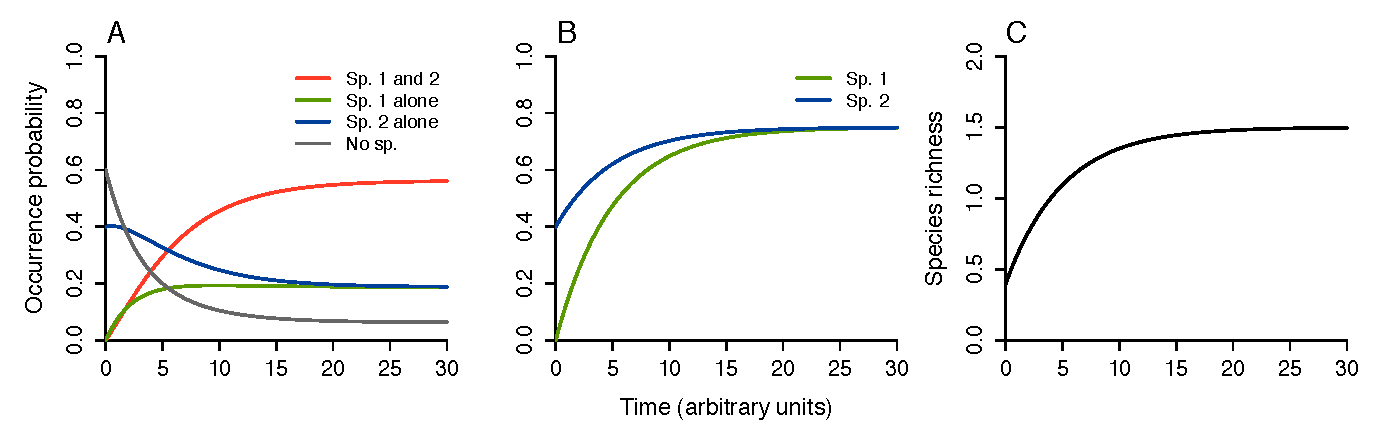
\includegraphics[width=\textwidth]{./annexe3/fig1.eps}
\caption[Simple food webs illustrating the TTTIB]{Simple food webs used to illustrate the TTTIB \cite{Gravel2011}.
 (a) The complete food web (on the mainland) consists in five different species (A, B, C, D, E);
 (b) sub-food webs that species A can colonize; (c) sub-food webs that species A cannot colonize.
}
\label{ann3fig1}
\end{figure}

\section{Reasonable approximations}\label{reasonable-approximations}

The formulation above allows the study of assemblages of non-independent species
but suffers from its generality: for \(T\) species, the
matrix \(\mathbf{M}\) must be filled out with \((2^T-1) \times (2^T-1)\)
coefficients (`\(-1\)' acknowledges that for any time \(t\) the elements
of \(\mathbf{P}(t)\) sum to one). Even if the knowledge of a particular
network may help finding these coefficients, reasonable assumptions can
be made to decrease the complexity of \(\mathbf{M}\). First, community
compositions between \(t\) and \(t+dt\) cannot differ in more than one
species, \emph{i.e.} \(f(S_k,S_l)=0\) if \(|S_k-S_l|>1\). This turns
\(\mathbf{M}\) into a sparse matrix: only \(T \times (2^T-1)\) are not
zero. This assumption is not possible in the TTIB as the extinction of a
prey leads to more than one extinction. However, this issue is easy
to circumvent by allowing the predator to survive a (very) short period
alone one the island which would be assumed using large value for
\(f(S_k,S_l)\) that measures the transition of a community with a
predator and the same community without it.

A second hypothesis is that colonization processes may be independent of
interactions. That is, a predator may actually colonize an island
without any prey. This is reasonable if the extinction probability of
this predator on such island is high. Therefore, \(f(S_k,S_l)=c\)
when \(sum\{S_k-S_l\}=-1\). The latter assumption is also useful to
integrate variability among species' dispersal capacities \citep{Cazelles2016a}.
Tables \ref{tabAnnIII_3} and \ref{tabAnnIII_4} present the matrix
\(\mathbf{M}\) for species C, D and E, \emph{i.e.} community
states from \(S_0\) to \(S_8\). Once the colonization probability is
determined, the remaining \(T \times (2^T-2)\) coefficients needed can
be found based on the biological knowledge of species studies,
\emph{e.g.} the nature and the strength of interactions.



\section{Deriving species richness}\label{deriving-species-richness}

The solution \(\mathbf{P}^{\*}\) includes the probabilities of all
community states at equilibrium. This information is more than
the knowledge of individual presences and species richness.
In order to obtain the probability of species $i$ being present on the island
at equilibrium, the following sum of probabilities is computed:

\begin{equation}
P_{X_i=1} = \sum_{k \mid S_{k,i}=1} \mathbf{P}_{k}^{\*}
\end{equation}

where \(S_{i,k}\) is the \(i^{th}\) component of \(S_i\) (the one
pertaining to species \(i\)) and \(\mathbf{P}_{i}^{\*}\) the \(k^{th}\)
component of \(\mathbf{P}_{i}\). Similarly, the species richness is
given by the sum of \(\mathbf{P}^{\*}\) weighted by the cardinal of the
community states it refers to:

\begin{equation}
S= \sum_{k=0}^{2^T-1} |S_k|\mathbf{P}_{k}^{\*}
\end{equation}

In a similar fashion, many probabilities can be derived regarding either
a particular set of species either a particular property of the
community. For instance, this framework allows to derive the probability
of finding a given set of predators but also the mean trophic level
expected and even the probability of having a trophic chains of at least
\(p\) levels. In all these situations, calculus necessitate the
identification of the community states to be summed.


\newpage

\begin{landscape}

  \begin{longtable}[]{@{}llllll@{}}
  \caption[Transition matrix of the continuous-time Markov chain (part 1/2)]{The transition matrix of the continuous-time Markov chain
  associated to all combinations of C, D and E species (part 1/2). An empty cell means 0.}\tabularnewline
  \toprule
  & \(S_{0}\) & \(S_{1}\) & \(S_{2}\) & \(S_{3}\) &
  \(S_{4}\)\tabularnewline
  \midrule
  \endhead
  \(S_{0}\) & \(1-c-c-c\) & \(f(S_{1},S_{,0})\) & \(f(S_{2},S_{,0})\) & &
  \(f(S_{4},S_{,0})\)\tabularnewline
  \(S_{1}\) & \(c\) & \(1-f(S_{1},S_{,0})-c-c\) & & \(f(S_{3},S_{,1})\)
  &\tabularnewline
  \(S_{2}\) & \(c\) & & \(1-f(S_{2},S_{,0})-c-c\) & \(f(S_{3},S_{,2})\)
  &\tabularnewline
  \(S_{3}\) & & \(c\) & \(c\) & \(1-f(S_{3},S_{,1})-f(S_{3},S_{,2})-c\)
  &\tabularnewline
  \(S_{4}\) & \(c\) & & & & \(1-f(S_{4},S_{,0})-c-c\)\tabularnewline
  \(S_{5}\) & & \(c\) & & & \(c\)\tabularnewline
  \(S_{6}\) & & & \(c\) & & \(c\)\tabularnewline
  \(S_{7}\) & & & & \(c\) &\tabularnewline
  \bottomrule
  \label{tabAnnIII_3}
  \end{longtable}


\end{landscape}


\newpage

\begin{landscape}

  \begin{longtable}[]{@{}llll@{}}
  \caption[Transition matrix of the continuous-time Markov chain (part 2/2)]{The transition matrix of the continuous-time Markov chain
  associated to all combinations of C,D and E species (part 2/2). An empty cell means 0.}\tabularnewline
  \toprule
  & \(S_{5}\) & \(S_{6}\) & \(S_{7}\)\tabularnewline
  \midrule
  \endhead
  \(S_{0}\) & & &\tabularnewline
  \(S_{1}\) & \(f(S_{5},S_{,1})\) & &\tabularnewline
  \(S_{2}\) & & \(f(S_{6},S_{,2})\) &\tabularnewline
  \(S_{3}\) & & & \(f(S_{7},S_{,3})\)\tabularnewline
  \(S_{4}\) & \(f(S_{5},S_{,4})\) & \(f(S_{6},S_{,4})\) &\tabularnewline
  \(S_{5}\) & \(1-f(S_{5},S_{,1})-f(S_{5},S_{,4})-c\) & &
  \(f(S_{7},S_{,5})\)\tabularnewline
  \(S_{6}\) & & \(1-f(S_{6},S_{,2})-f(S_{6},S_{,4})-c\) &
  \(f(S_{7},S_{,6})\)\tabularnewline
  \(S_{7}\) & \(c\) & \(c\) &
  \(1-f(S_{7},S_{,3})-f(S_{7},S_{,5})-f(S_{7},S_{,6})\)\tabularnewline
  \bottomrule
  \label{tabAnnIII_4}
  \end{longtable}


\end{landscape}


\newpage
